\documentclass{beamer}
\begin{document}
\title{Introduction to\\KiCAD \& Open Hardware}
\author{Katharina Fey}
\date{17. March 2018}

\frame{\titlepage}


%%%%%%%%%%%%%%%%%%%%%%%%%%%%%%%%%%%%%%%%%%%%%%%%%%%%%%%%%
\begin{frame}
  \frametitle{Contents}
  \begin{itemize}
    \item Introduction
    \begin{itemize}
      \item What is hardware development
      \item What is KiCAD?
    \end{itemize}
    \item Workflow
    \begin{itemize}
      \item Creating schematic symbols
      \item Creating footprints
      \item Working with schematics and boards
      \item Updating designs
    \end{itemize}
    \item Project Management
    \begin{itemize}
      \item Datasheets
      \item Multiple schematic files
      \item Library/ Parts management
    \end{itemize}
  \end{itemize}
\end{frame}


%%%%%%%%%%%%%%%%%%%%%%%%%%%%%%%%%%%%%%%%%%%%%%%%%%%%%%%%%
\begin{frame}
  \frametitle{Introduction}
  \begin{itemize}
    \item Components, Boards and Firmware
    \item Open Hardware addresses entire stack
    \item Board (PCB) design is "drawing"
  \end{itemize}

  \begin{figure}[H]
    \centering
    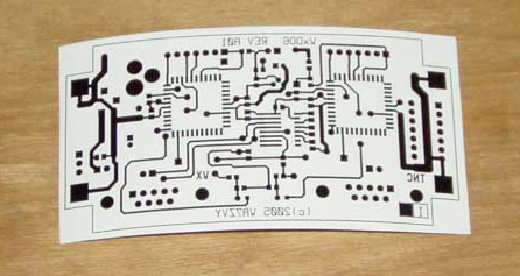
\includegraphics[width=0.45\textwidth]{images/pcb_on_paper.jpg}
    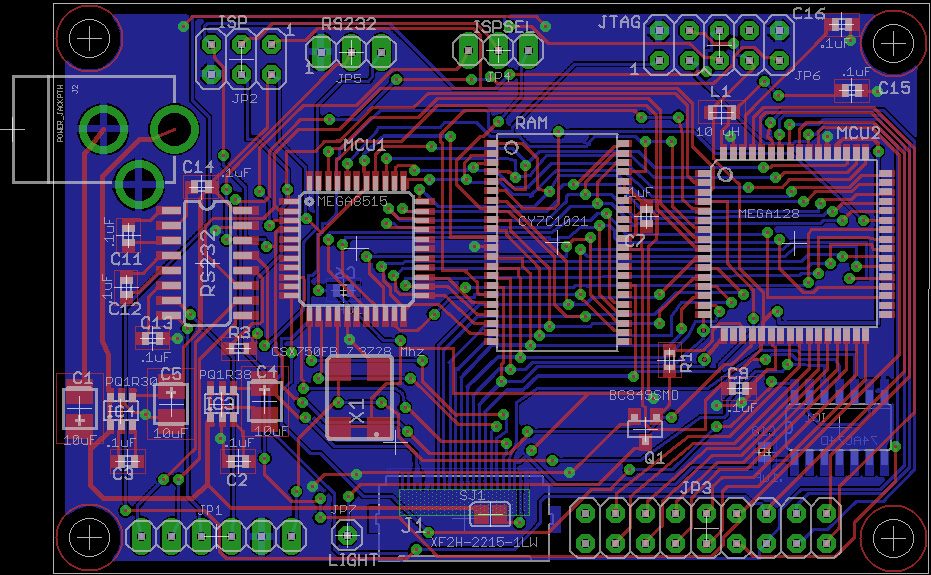
\includegraphics[width=0.45\textwidth]{images/pcb_in_kicad.jpg}
  \end{figure}

\end{frame}


%%%%%%%%%%%%%%%%%%%%%%%%%%%%%%%%%%%%%%%%%%%%%%%%%%%%%%%%%
\begin{frame}
  \frametitle{KiCAD}
  \begin{itemize}
    \item Developed by CERN
    \item Current version 4.0.*
    \item Next version (5.0) just around the corner
    \item Open ecosystem around components \& footprints
  \end{itemize}
\end{frame}


%%%%%%%%%%%%%%%%%%%%%%%%%%%%%%%%%%%%%%%%%%%%%%%%%%%%%%%%%
\begin{frame}
  \frametitle{Workflow}
  \begin{itemize}
    \item Schematics (represent Circuits)
    \item Associate Footprints
    \item Layout boards \& route traces
    \item Repeat for iterations
  \end{itemize}

  \begin{figure}[H]
    \centering
    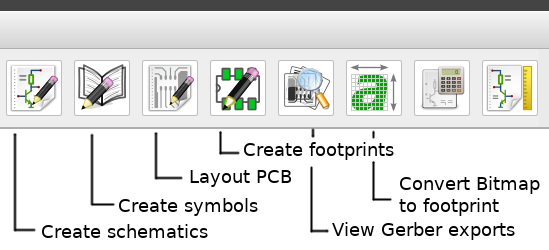
\includegraphics[width=0.95\textwidth]{images/workflow_overview.png}
  \end{figure}

\end{frame}


%%%%%%%%%%%%%%%%%%%%%%%%%%%%%%%%%%%%%%%%%%%%%%%%%%%%%%%%%
\begin{frame}
  \frametitle{Schematics}
  \begin{itemize}
    \item Symbols (Create missing symbols)
    \item Labels
    \item Connections
  \end{itemize}

  \begin{figure}[H]
    \centering
    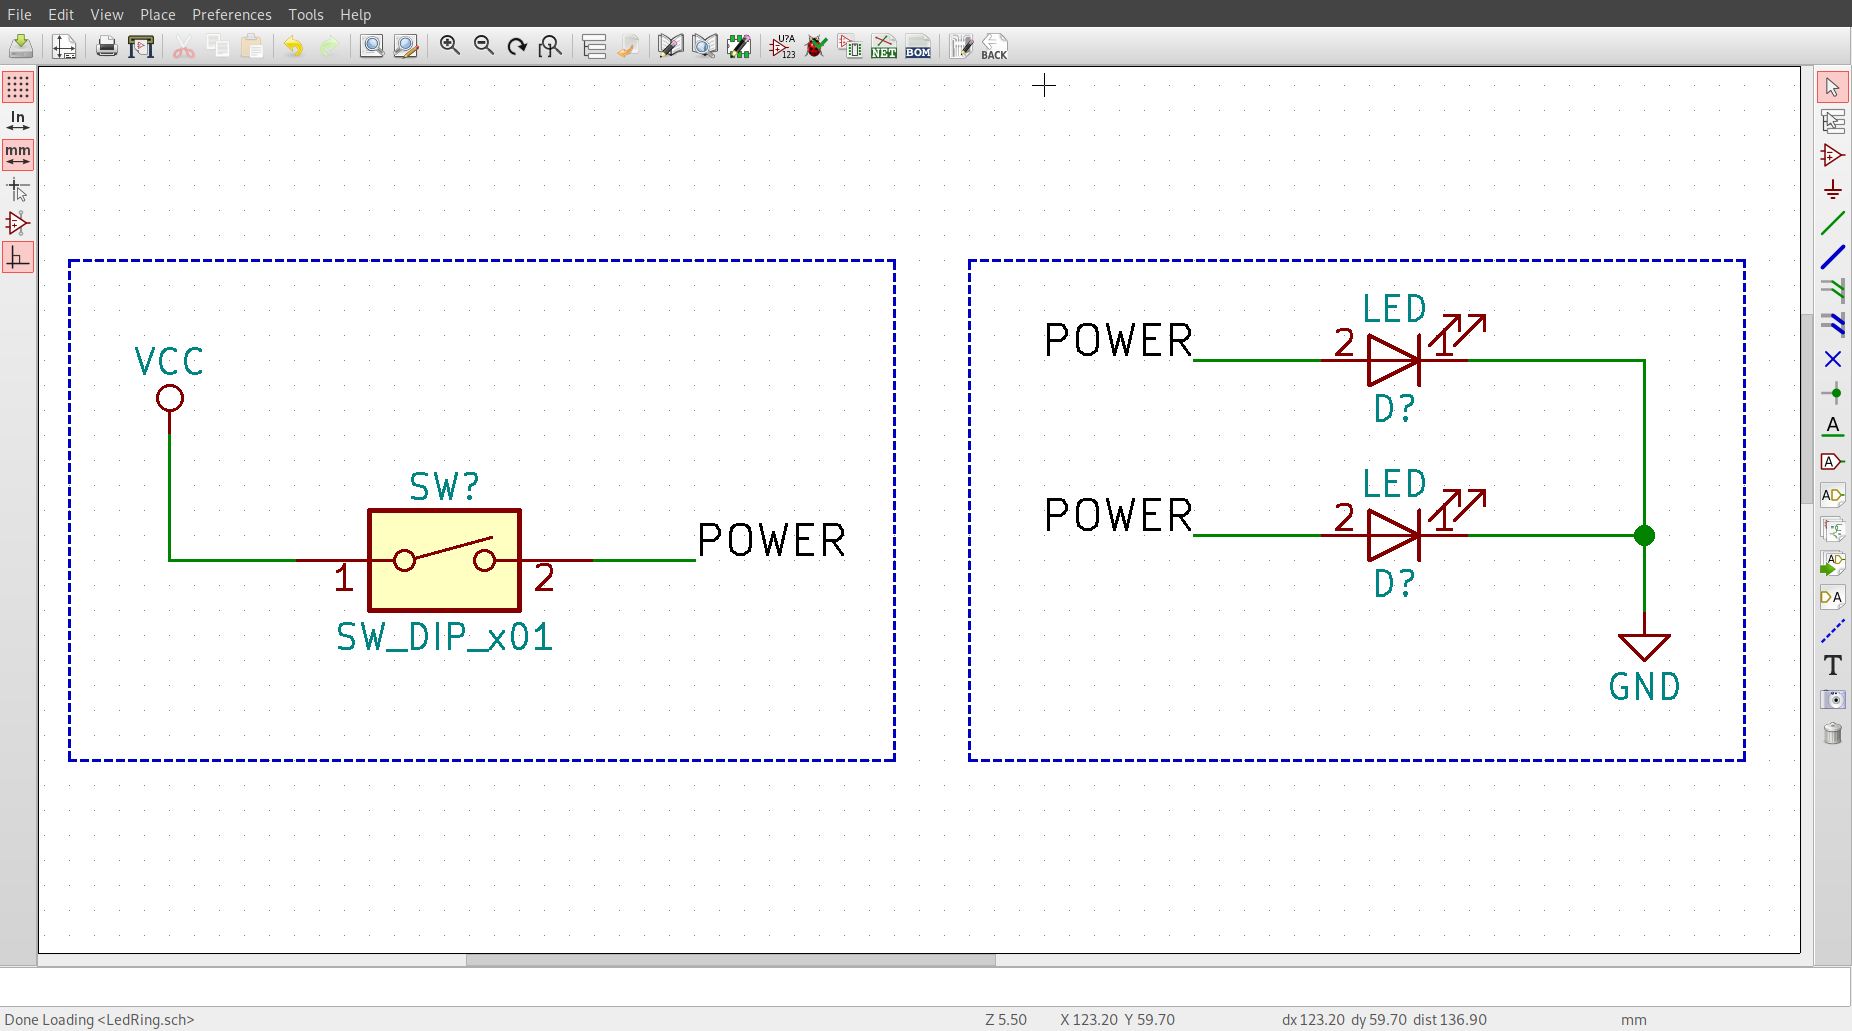
\includegraphics[width=0.95\textwidth]{images/kicad_schematic.png}
  \end{figure}

\end{frame}


%%%%%%%%%%%%%%%%%%%%%%%%%%%%%%%%%%%%%%%%%%%%%%%%%%%%%%%%%
\begin{frame}
  \frametitle{Schematics Workflow}
  \begin{itemize}
    \item Create circuit schematic
    \item Annotate (Give components unique names)
    \item Associate footprints
    \item Export Netlist
  \end{itemize}
\end{frame}


%%%%%%%%%%%%%%%%%%%%%%%%%%%%%%%%%%%%%%%%%%%%%%%%%%%%%%%%%
\begin{frame}
  \frametitle{Board Layout}
  \begin{itemize}
    \item Import Netlist
    \item Layout components
    \item Route traces
    \item Export
  \end{itemize}
\end{frame}


%%%%%%%%%%%%%%%%%%%%%%%%%%%%%%%%%%%%%%%%%%%%%%%%%%%%%%%%%
\begin{frame}
  \frametitle{Understanding Datasheets}
  \begin{itemize}
    \item Describes a component in detail
    \item Not everything always relevant
    \item Pick out important information
    \begin{itemize}
      \item High-level description
      \item Example usage
      \item Pin-out
      \item Footprint size
    \end{itemize}
  \end{itemize}
\end{frame}



\end{document}

